%% \documentclass[a4paper]{article}
%% \usepackage{pgfplots}
%% \pgfplotsset{compat=1.16}
%% \begin{document}

\begin{tikzpicture}
\begin{semilogxaxis}[
%  title = Experiment on the time taken to find a bug,
  ylabel = Time (ms),
  xlabel = Invocations per thread,
  % ymax = 4,
  log basis x=2,
  scaled ticks = false,
  legend pos = north west,
  height = 0.4\textheight,
  width = 0.90\textwidth
]
\addplot+[error bars/.cd, y dir=both,y explicit] coordinates {
  (2,83.08509326000001) +- (0,1.2354531362387784)
  (4,74.88299255) +- (0,1.3112835057583532)
  (8,79.067596255) +- (0,1.9395745438227188)
  (16,80.47892682999999) +- (0,2.0364739691984073)
  (32,80.797998155) +- (0,1.8239378697908442)
};
\addlegendentry{$p = 2$}
\addplot+[error bars/.cd, y dir=both,y explicit] coordinates {
  (2,87.516821685) +- (0,1.4792666407834463)
  (4,81.817856485) +- (0,1.651014381813079)
  (8,84.73854852) +- (0,2.6680012145096885)
  (16,89.37923438) +- (0,2.1757320329956484)
  (32,95.14338612) +- (0,2.828884694709013)
};
\addlegendentry{$p = 4$}
\addplot+[error bars/.cd, y dir=both,y explicit] coordinates {
  (2,94.39215556) +- (0,2.1871718235223345)
  (4,89.20503961) +- (0,1.423227793928453)
  (8,97.728336265) +- (0,2.663437124298785)
  (16,106.08867011) +- (0,3.660762475944014)
  (32,117.08226379000001) +- (0,3.54637813404394)
};
\addlegendentry{$p = 8$}
\addplot+[error bars/.cd, y dir=both,y explicit] coordinates {
  (2,99.684097325) +- (0,2.1639888413012356)
  (4,101.14500844499999) +- (0,1.1203456199995476)
  (8,115.256713) +- (0,3.5984690955172924)
  (16,122.60207184000001) +- (0,1.190600621017305)
};
\addlegendentry{$p = 16$}
\end{semilogxaxis}
\end{tikzpicture}

% --samples 200 --tester ChanTester --maxItersPerRun 256
%\end{document}
